\documentclass[letterpaper, 12pt]{article}
\usepackage{fullpage,latexsym,amsthm,latexsym,amssymb}
\usepackage{amstext,amsfonts,amsmath,graphicx}
\usepackage{multicol}
\usepackage[usenames,dvipsnames]{color}
\usepackage{hyperref}
\usepackage{tikz}
\usepackage{graphicx}
\graphicspath{./} 
\usetikzlibrary{automata, positioning}

\oddsidemargin = -0.5 in
\addtolength{\textwidth}{0.8in}
\addtolength{\textheight}{0.2in}

%% Theorem statements %%
% THEOREMS -------------------------------------------------------
\newtheorem{theorem}{Theorem}[section]
\theoremstyle{definition}
\newtheorem{definition}{Definition}
\numberwithin{equation}{section}
%% MISC DEFINITIONS %%%%%%%%%%%%%%%%%%%%%%%%%%%%%%%%%%%

\newcommand{\ignore}[1]{}

\DeclareMathOperator{\shuffle}{shuffle}

\newcommand{\N}{\mathbb N}
\newcommand{\abs}[1]{\left \vert #1 \right\vert}
\newcommand{\abi}[1]{\textcolor{Red}{#1}}
\newcommand{\qtrinfo}{CS181 Winter 2019}
\newcommand{\remove}[1]{}
\newcommand{\headnote}{
%\begin{multicols}{2}\small
\begin{itemize}
\item Please write your student ID \textbf{and the names of anyone you collaborated with} in the spaces provided and attach this sheet to the front of your solutions. \textbf{Please do not include your name anywhere since the homework will be blind graded.}
\item An extra credit of \textbf{5\%} will be granted to solutions written using \LaTeX. Here is one place where you can create \LaTeX documents for free: \url{https://www.sharelatex.com/}. The link also has tutorials to get you started. There are several other editors you can use.
\item If you are writing solutions by hand, please write your answers in a neat and readable hand-writing.
\item Always explain your answers. When a proof is requested, you should provide a rigorous proof.
\item If you don't know the answer, write ``I don't know'' along with a clear explanation of what you tried. For example: ``I couldn't figure this out. I think the following is a start, that is correct, but I couldn't figure out what to do next. [[Write down a start to the answer that you are sure makes sense.]] Also, I had the following vague idea, but I couldn't figure out how to make it work. [[Write down vague ideas.]]'' At least 20\% will be given for such an answer.

Note that if you write things that do not make any sense, no points will be given.
\item The homework is expected to take anywhere between 8 to 14 hours. You are
advised to start early.
\item Submit your homework online on the course webpage on CCLE. You can also hand it in at the end of any class before the deadline.
\end{itemize}
%\end{multicols}
}

\newcommand{\hwhead}[2]{
	\raggedleft{Student ID: \underline{\hspace{1.2in}304990072\hspace{1.25in}} \\ \medskip
              Collaborators: \underline{\hspace{3in}} \\ \medskip}
  \bigskip
  \begin{center}
  	{\LARGE{\qtrinfo \ -- Problem Set #1}}\\[0.3cm]
  	{\Large{Due #2}}
  \end{center}
  \bigskip
  \raggedright
  \headnote
}

%%%%%%%%%%%%%%%%%%%%%%%%%%%%%%%%%%%%%%%%%%%%%%%%%%%%%
\addtolength{\topmargin}{-1cm}
\addtolength{\textheight}{2cm}






\begin{document}
\hwhead{2}{Tuesday, February 5, 11:59 pm}


\begin{center}
\fbox{%
   \parbox{0.8\linewidth}{
Note: \textit{All questions in the problem sets are challenging; you should not expect to know how to answer any question before trying to come up with innovative ideas and insights to tackle the question. If you want to do some practice problems before trying the questions on the problem set, we suggest trying problems 1.17 and 1.23 from the book. Do not turn in solutions to problems from the book.}
   }%
}
\end{center}


\newpage
\paragraph{Problem 1}
\subparagraph{} Assume not. That is, both shuffle$(L_1,L_2)$ and shuffle$(L_1, \overline{L_2})$ are regular. Since the class of regular languages is closed under the union operation, shuffle$(L_1,L_2)$ $\cup$ shuffle$(L_1, \overline{L_2})$ is regular. That is, $L = \{x_1y_1x_2y_2\ ...\ x_ny_n\ |\ x_1\ ...\ x_n \in L_1,\ y_1...y_n \in \Sigma ^*\}$ = shuffle $(L_1,\Sigma^*)$. We have proved in the discussion that $L_{alt} = \{x\ |\ \exists y \in L\ such\ that\ x_1x_2x_3...=y_1y_3y_5...\}$ is regular if $L$ is regular. Since $L =$ shuffle $(L_1,\Sigma^*)$ is regular in this case, $L_1$ is regular, which is a contradiction as we are given $L_1$ is not regular. Hence, the languages shuffle$(L_1,L_2)$ and shuffle$(L_1, \overline{L_2})$ cannot both be regular. (proven)
\\~\\

\newpage
\paragraph{Problem 2}
\subparagraph{(a)}
for any $w \in L_2 = L_1 \cup b^* $, $|w|\geq1$, Let $q=1$\\~\\
\begin{itemize}
	\item $w \in L_1$. Let $x=\epsilon,\ y=a,\ z=a^{i-1}b^p$. Thus, for each $w \in L_1$, we can write $w=xyz$, and $|xy| = 1 = q,\ |y|=1>0$. \\
	$\Rightarrow$ $xy^jz \in L_1$ if $j >0$,  $xy^iz \in b^*$ if $j=0, i=1$.\\
	$\Rightarrow$ $xy^jz \in L_2$
	\item $w \in b^*$. Let $x=\epsilon,\ y=b,\ z=b^{|w|-1}$. Thus, for each $w \in b^*$, we can write $w=xyz$, and $|xy| = 1 = q,\ |y|=1>0$. \\
	$\Rightarrow$ $xy^jz \in b^*$ for $j\geq0$.
\end{itemize}    
Hence, $L_2$ satisfies the conditions of the Pumping Lemma. (proven)

\subparagraph{(b)} Since $L$ is a regular language, there exists a DFA $M_1$ that accepts $L$. Assume that there are $q$ states in the DFA. Let $w=w_1w_2w_3...w_n$, where $n \geq q$. Let $r_1r_2...r_nr_{n+1}$ be the sequence of states $M_1$ enters for the input string $w$, so $r_{i+1}=\delta(r_i,w_i)$ for $1 \leq i \leq n$. For any partition of $w = xyz,\ y \geq q$, $M_1$ enters the state of $r_{|x|+1}$ after processing string x. Then $M_1$ continues to process $y$ which has at least $q$ states. Thus, after finishing processing $y$, $M_1$ will go through at least another $q+1$ states including $r_{|x|+1}$. Since there are only q states in the DFA, by Pigeonhole Principle, at least two of the states must be the same. We denote the first of these by $r_j$, the second by $r_l$ ($ j \neq l$). Let $b$ be the string that makes $M_1$ enter $r_l$ from $r_j$ ($r_j=r_l$), $a$ be the string that makes $M_1$ enter $r_j$ from $r_{|x|+1}$, $c$ be the remaining part of string $y$. Thus, after process the string $xa$, $M_1$ enters the state $r_j$, and any number of string $b$ input after $xa$ will make $M_1$ re-enter $r_j/r_l$. And string $cz$ will make $M_1$ to enter an accepted state from $r_j/r_l$, since $w=xyz$ is accepted by $L$. Hence, we have proved for every $w \in L$, and every partition of $w$ into $w=xyz$ with $|y| \geq q$, there are strings $a, b, c$ such that $y=abc$, $|b| > 0$, and for all $i\geq0$, $xab^icz \in L$. (proven)

\subparagraph{(c)} Assume not. Consider a string $w=a^qb^p$, $p$ is a prime and $p > q$. Hence $w\in L_2$. Let $x = a^q,\ y=b^q,\ z =b^{p-q}$ be a partition of $w$. Clearly if $L_2$ is a regular language, there exists a partition $y=rst,\ |s| >0$, such that for all $i \geq 0$, $xrs^itz \in L_2$. Since $y =b^q$, $s$ must be in the form of $b^j$, $0<j\leq q$. Thus, $xrs^itz = a^qb^{p+(i-1)j}$, and there exists a $j$ such that $p+(i-1)j$ is a prime regardless the value of $i$. However, when $i-1 = p$, $p+(i-1)j= p+pj=p(j+1)$ which is not a prime. This is a contradiction. Hence, $L_2$ is not a regular language. (proven)
\newpage
\paragraph{Problem 3}
\subparagraph {}
Assume not. Consider $L_1=0^*21^*$. $L_2$ is a regular language as we can easily find out that it is accepted by the following state machine:
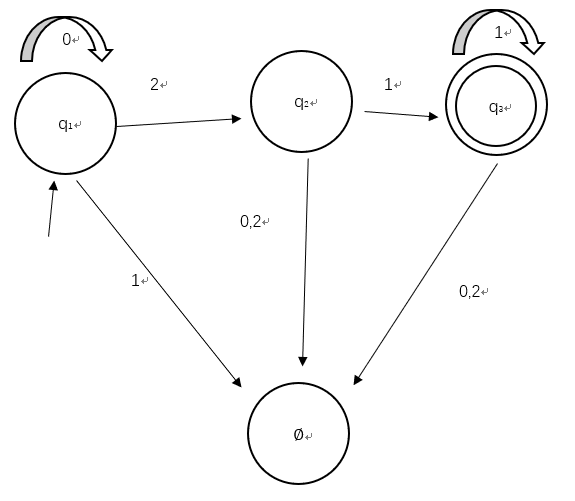
\includegraphics{statemachine_1} \\
Let $L_{\frac{1}{3}-\frac{1}{3}} = \{xz \in \Sigma^*\ |\ \exists y \in \Sigma^*\  with\  |x|=|y|=|z|\ such\ that\ xyz \in L\}$. In this case, we let $L = L_1, \Sigma = \{0,1,2\}$, and $L_{\frac{1}{3}-\frac{1}{3}}$ is a regular language. \\~\\
Now, consider another language $L_2 = 0^*1^*$, it is also fairly easy to prove that $L_2$ is a regular language by introducing the following state machine:
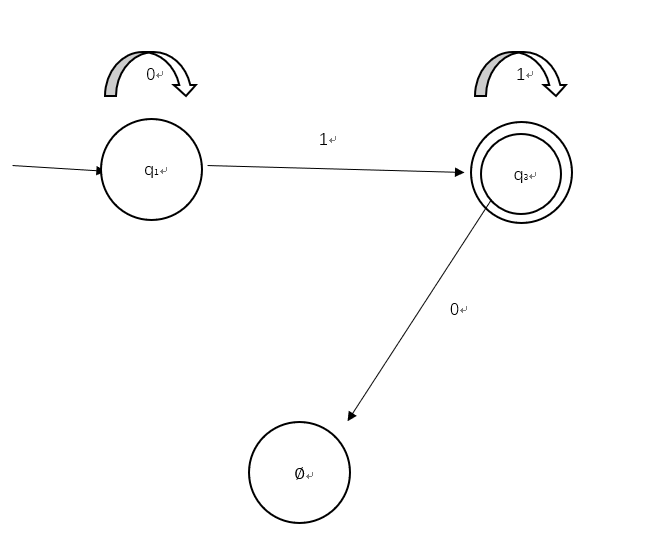
\includegraphics{statemachine_2} \\
Since the class of regular languages is closed under the union operation,  $L_3 = L_{\frac{1}{3}-\frac{1}{3}} \cup L_2$ is a regular language by our construction. \\~\\

Now let's prove $L_3 = 0^i1^i,\ i > 0$. Assume not. Since $L_3 = L_{\frac{1}{3}-\frac{1}{3}} \cup L_2$, $L_2 = 0^*1^*$, there is no alphabet "2" in $L_3$. Since $L_{\frac{1}{3}-\frac{1}{3}} = \{xz \in \Sigma^*\ |\ \exists y \in \Sigma^*\  with\  |x|=|y|=|z|\ such\ that\ xyz \in L_1\}$, resulting that $L_3$ must satisfy $L_3 = 0^i1^j,\ i >0,j>0,\ i \neq j, (i+j)\ mod\ 2 = 0$. Without loss of generality, assume $i > j$, since $|x|=|z|=\frac{i+j}{2}$, $x = 0^{\frac{i+j}{2}},\ z = 0^\frac{i-j}{2}1^j $. However, this is a contradiction because no matter what string y is, $xyz$ is not in $L_1$ because there would be $0$ on the right hand side of "2". Hence, $L_3 = 0^i1^i,\ i > 0$. \\~\\

However, we have proved in lecture that $L_3 = 0^i1^i,\ i > 0$ is not a regular language, which is a contradiction. Hence, if $L$ is regular, $L_{\frac{1}{3}-\frac{1}{3}}$ need not be regular. (proven)

\end{document}
